\documentclass[]{auvsi_doc}
\setkeys{auvsi_doc.cls}{
	AUVSITitle={UGV Parachute Testing Description}
	%AUVSILogoPath={./logo.pdf]}
}

% include extra packages, if needed
\usepackage{longtable}
\usepackage{gensymb}
\usepackage{subcaption}


\begin{document}

\begin{AUVSITitlePage}
\begin{artifacttable}
\entry{CD-004, 0.1, 2018-10-30, Initial Draft, John Akagi, Kameron Eves}
% additional \entry{} commands for extra rows in the revision table, if needed
\end{artifacttable}
\end{AUVSITitlePage}

This artifact details the methods and results of our UGV drop system concepts. The parachute concepts were tested in high bay in the Engineering Research Lab. There is scaffolding that allowed us an apporximately 30 foot drop into a 20 foot by 10 foot area. Initial testing was done on the methods to measure the landing velocity of the payload and to get a basic understanding of what variables were important to control. After the initial testing, we decided to test a large parachute, a small parachute, and a small parachute with control fins on the payload since these seemed to have the largest impact on the precision of the drop and the landing speed. The large parachute was 48 inches in diameter with a 16 inch diameter spill hole. The small parachute was 30 inches in diameter with a 6 inch diameter spill hole. The fin design was comprised of two fins with a total surface area of 19.5 in\textsuperscript{2}.

We tested these three methods by dropping each one three times and recording the impact point. The payload weight for each drop was .711 kg.  During these drops, we controlled the position, shape, and orientation of the parachute to reduce any effects that would be caused by imperfections in the construction of our parachute. For the drop with the fins, the fins were both oriented at apporximately a 45\degree angle and oriented to try and offset the leftward drift of the small parachute. The parachute and setup for the parachute connections are shown in Figure \ref{fig:combined}. The results of the test are shown in Table \ref{table:results} and the drop locations are shown in Figure \ref{fig:locations}. 

\begin{figure}[h!]
\centering
   \begin{subfigure}{0.49\linewidth} \centering
     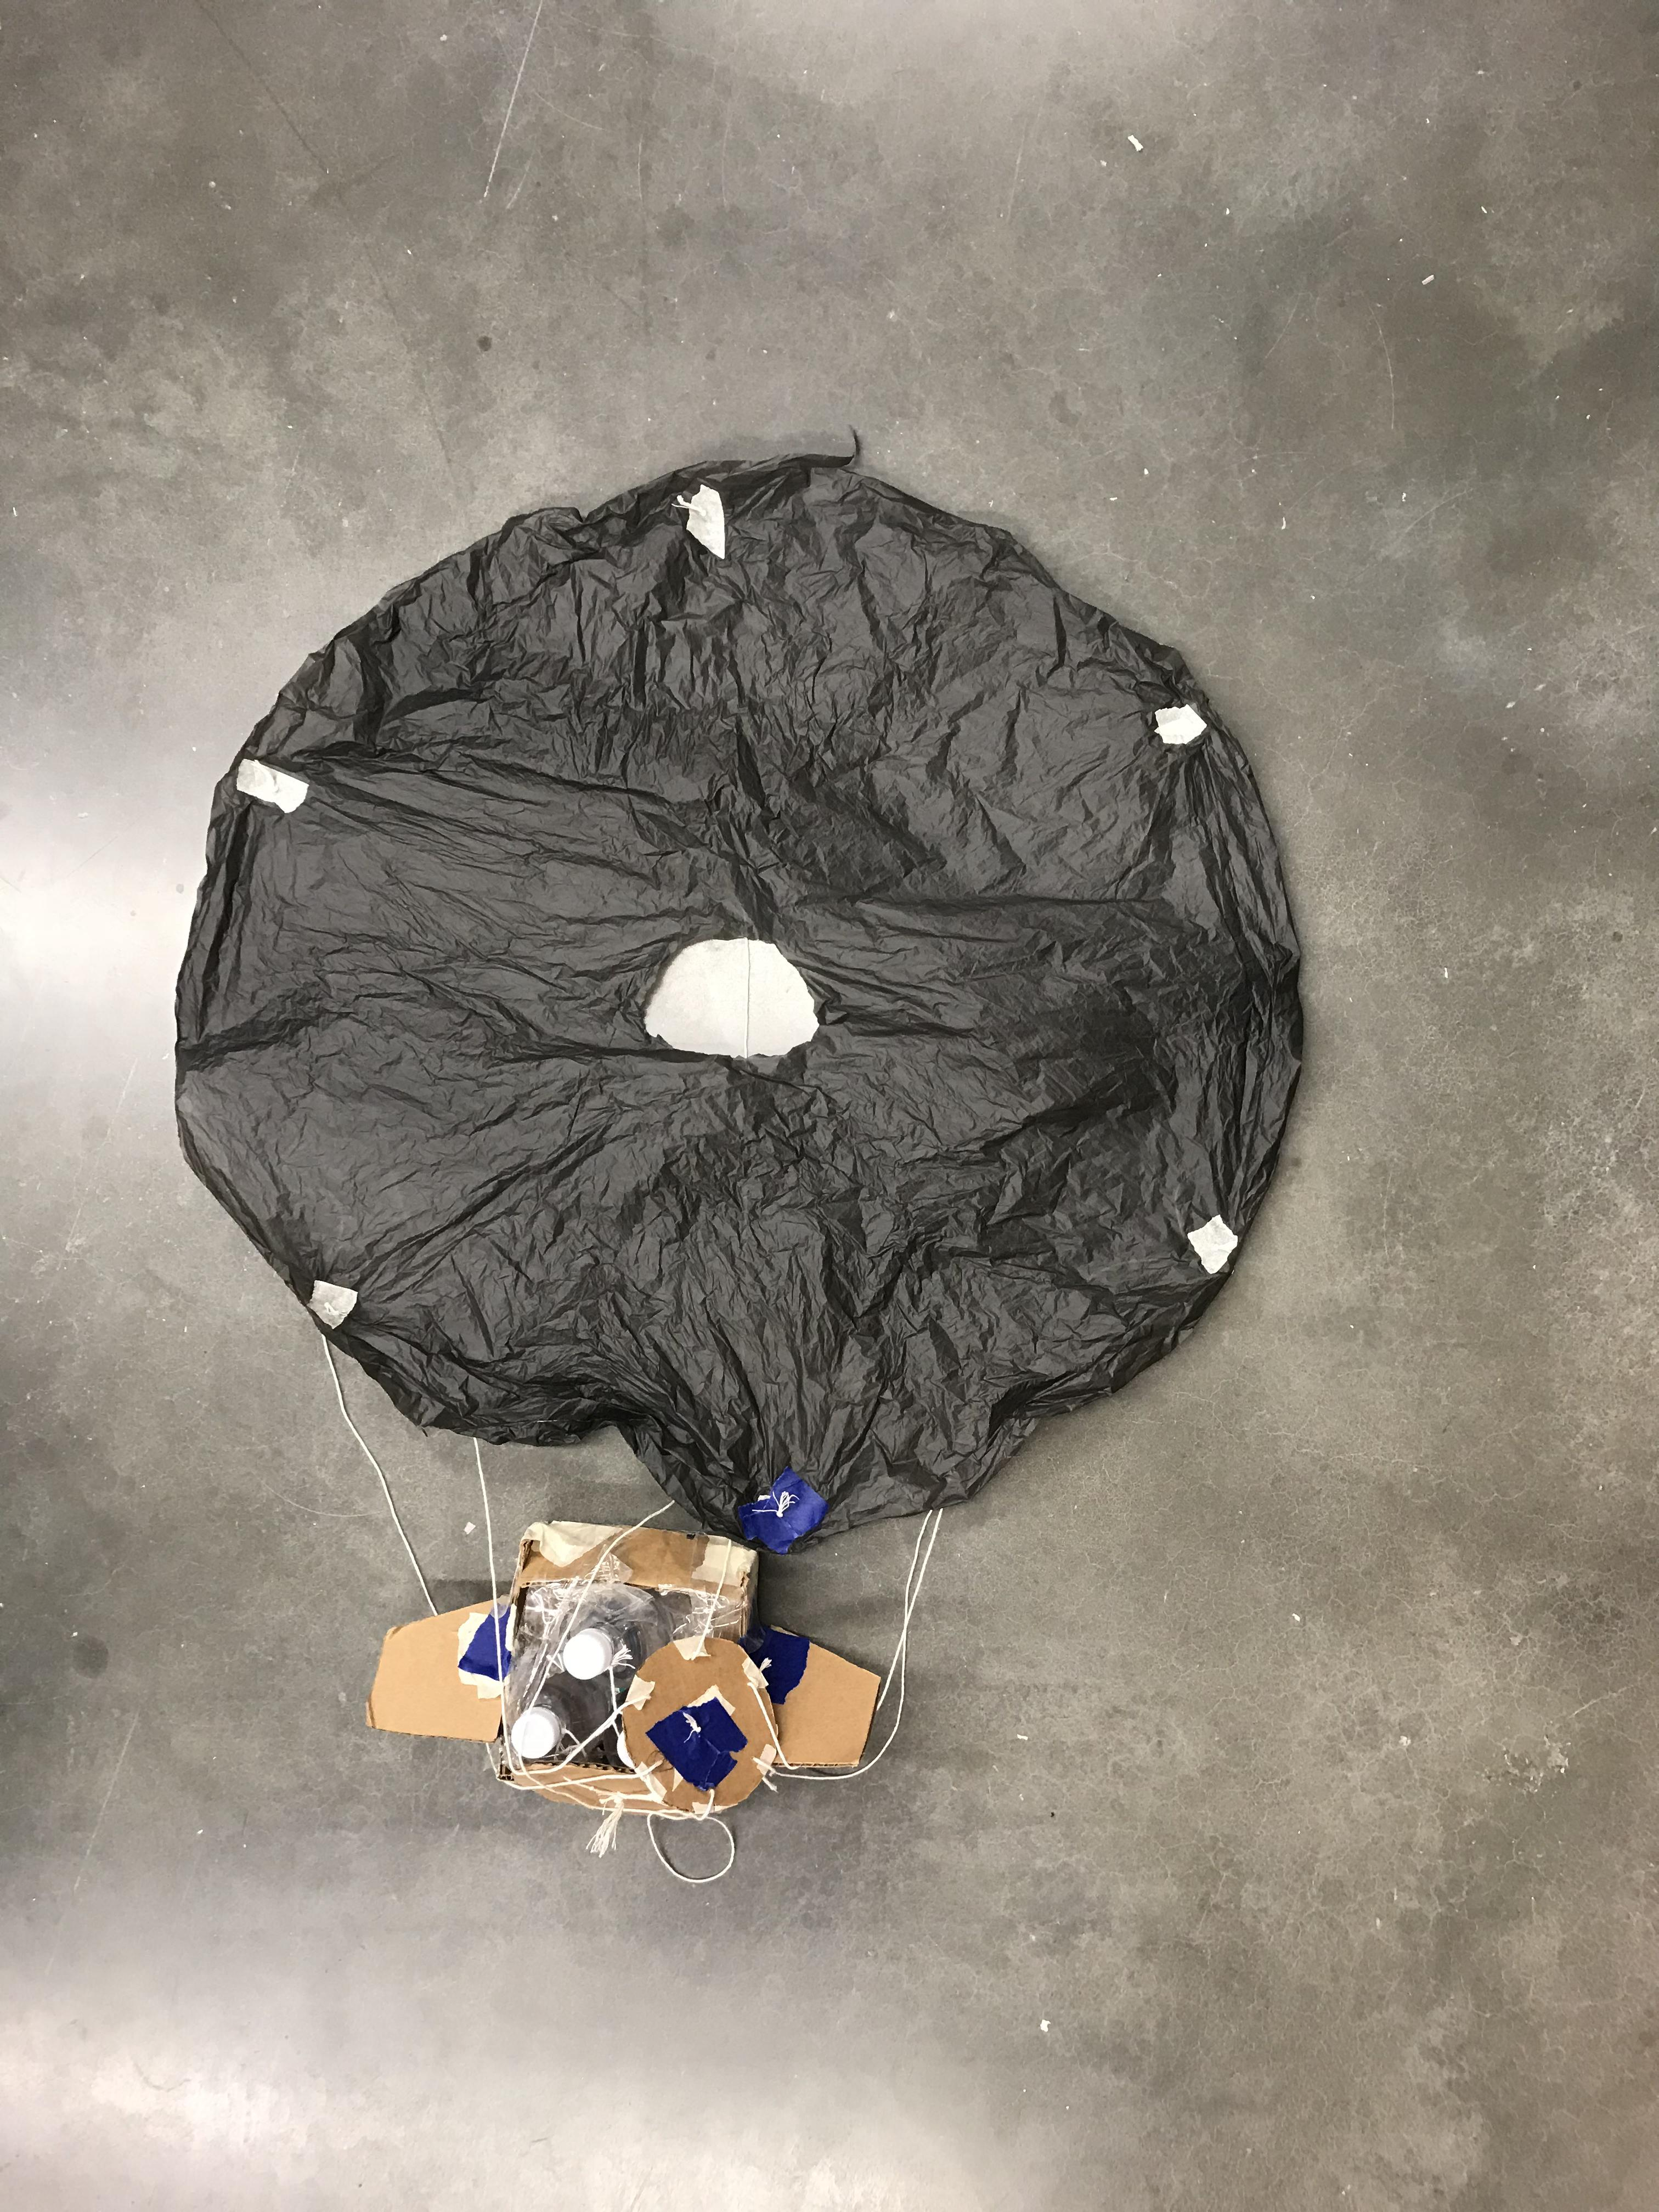
\includegraphics[width=.95\columnwidth]{Parachute1.jpg}
     \caption{Full configuration for parachute and fins.}\label{fig:fullParachute}
   \end{subfigure}
   \begin{subfigure}{0.49\linewidth} \centering
     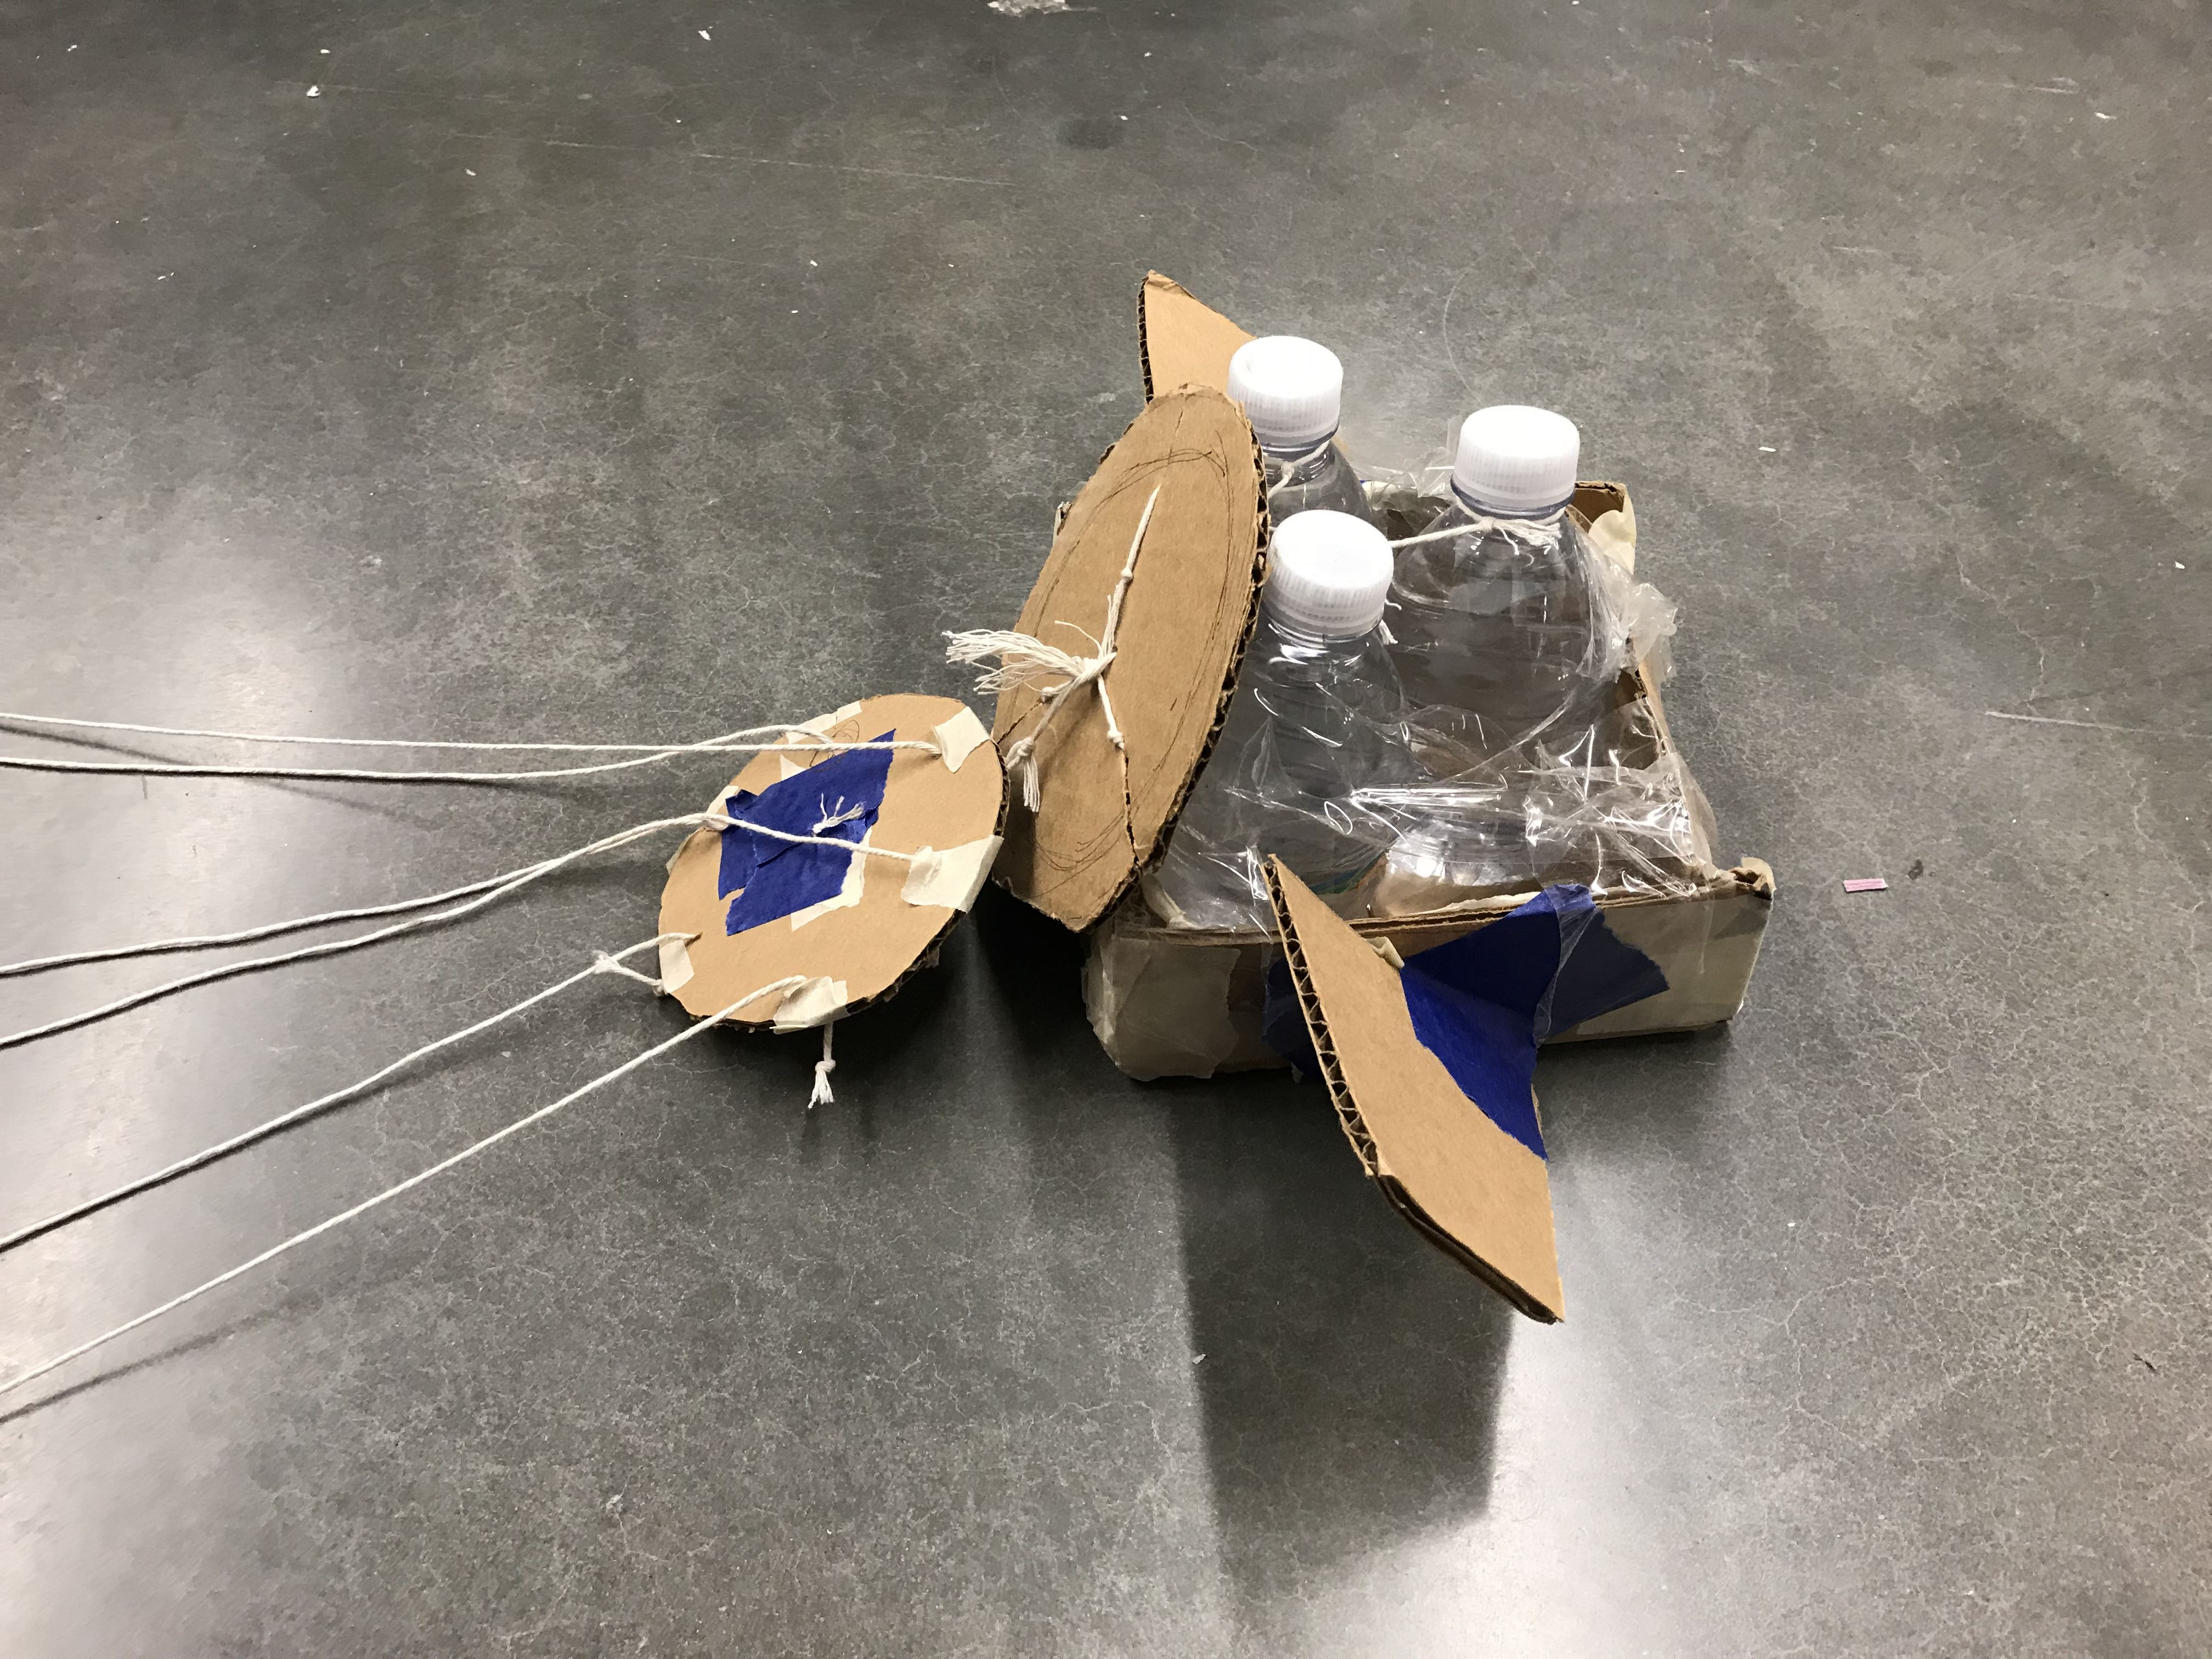
\includegraphics[width=.95\columnwidth]{Parachute2.jpg}
     \caption{Control fins and connections to parachute.}\label{fig:ControlFins}
   \end{subfigure}
\caption{Testing setup for the small parachute and fins option. The small parachute only method was the same but without the cardboard holder around the water bottles. The large parachute method was identical to the small parachute method but simply larger.} 
\label{fig:combined}
\end{figure}

\begin{table}[h]
\caption{The results of dropping the three different parachute systems. The average distance is the average distance between the point directly below where the parachute was dropped and the initial landing spot. The standard deviation is the standard deviation between all three drops for each system.}
\label{table:results}

\begin{tabular}{| l | l | l |}
\hline
Method & Average Distance & Std. Deviation\\
\hline
Large Parachute & 9.01 ft  & 0.95 ft\\
Small Parachute & 7.20 ft  & 1.38 ft\\
Small Parachute with Fins & 4.70  & 1.08 ft\\
\hline

\end{tabular}

\end{table}

\begin{figure}[h]
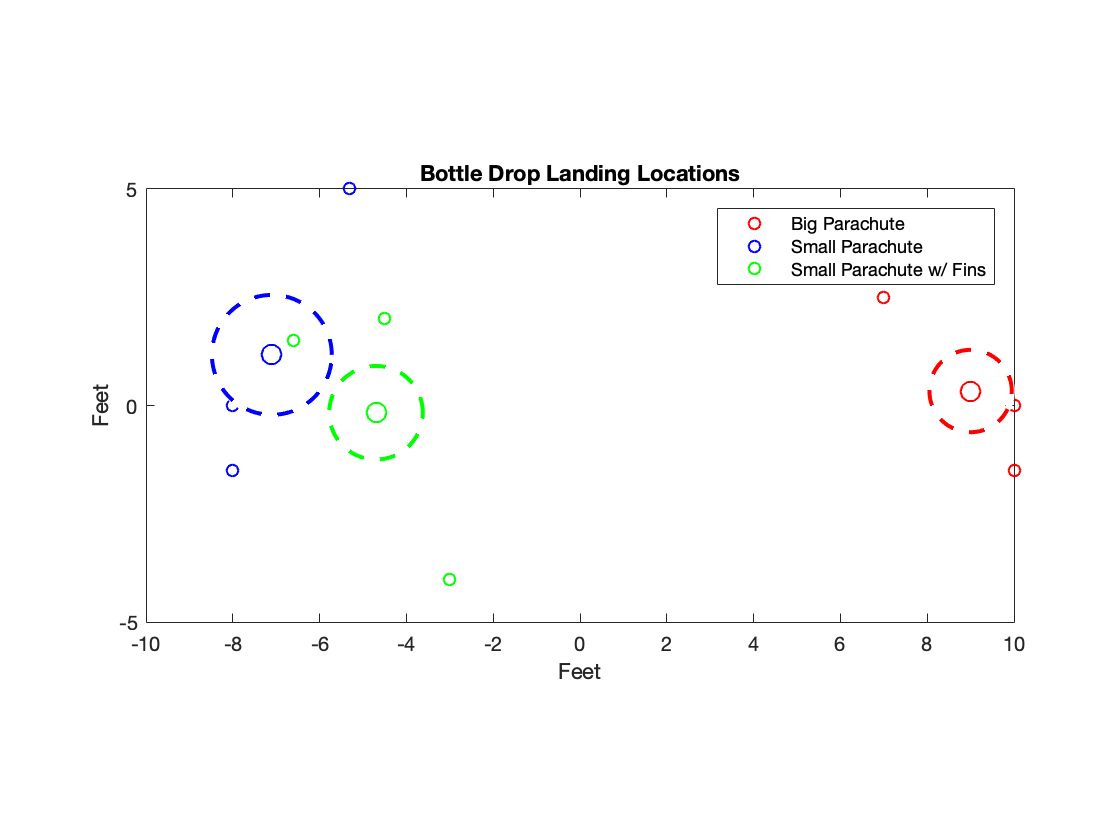
\includegraphics[width=\columnwidth]{LandingLocations.png}
\caption{The location of the initial impacts of each of the drops as shown by filled in circles. Due to the constrained area of our testing location, some landing locations were extrapolated since they hit the walls before the ground. The open circles are the average location of impact. The dashed lines indicate the mean distance away from the average impact location. The colors differentiate between system types as shown in the legend.}
\label{fig:locations}
\end{figure}





\end{document}
